\section{Petit historique du Raspberry Pi}

\begin{frame}
\frametitle{Pourquoi le Raspberry Pi ?}

\begin{itemize}
	\item de 1990 à 2000 baisse du niveau des adolescents en matière de codage et de connaissance des ordinateurs
	\item passage de l'ordinateur personnel à l'ordinateur familial
	\item d'où la volonté d'avoir un ordinateur à bas prix ``bidouillable''
\end{itemize}

Eben Upton, Robert Mullins, Jack Lang et Alan Mycroft en équipe avec Pete Lomas et David Braben ont créé la Fondation Raspberry Pi est l'équivalent d'une association de loi 1901 en France en 2009.

Il faudra attendre trois ans plus tard pour que la fabrication en série commence.

\end{frame}

\begin{frame}
\frametitle{Chronologie}
\begin{description}
	\item[Février 2012] Disponibilité  du Raspberry Pi A, le premier lot est vendu en quelques minutes
	\item[Mai 2012] La production atteint son rythme de croisière, le nombre de Pi par personne n'est plus de 1.
	\item[Septembre 2012] La fondation annonce que le Raspberry Pi sera désormais fabriqué en Angleterre
	\item[Octobre 2012] Le Raspberry Pi B est livré avec 512Mo
	\item[Février 2015] Sortie du Rapsberry Pi 2
	\item[Avril 2015] 5 millions de Raspberry Pi ont été vendus dont 500000 de Raspberry Pi 2
	\item[Novembre 2015] Le Rapsberry Pi Zéro est en vente. En rupture de stock en moins de 24 heures
	\item[Février 2016] Pour le quatrième anniversaire, le Raspberry Pi 3 apparaît
	\item[Septembre 2016] On en est à 10 millions de Raspberry Pi vendus
\end{description}
\end{frame}


\begin{frame}
\frametitle{la famille des Pis}
La famille des Pis est représentée sur cette image (figure \ref{img_family}) faite par RaspiTV.

\begin{center}
\begin{figure}
	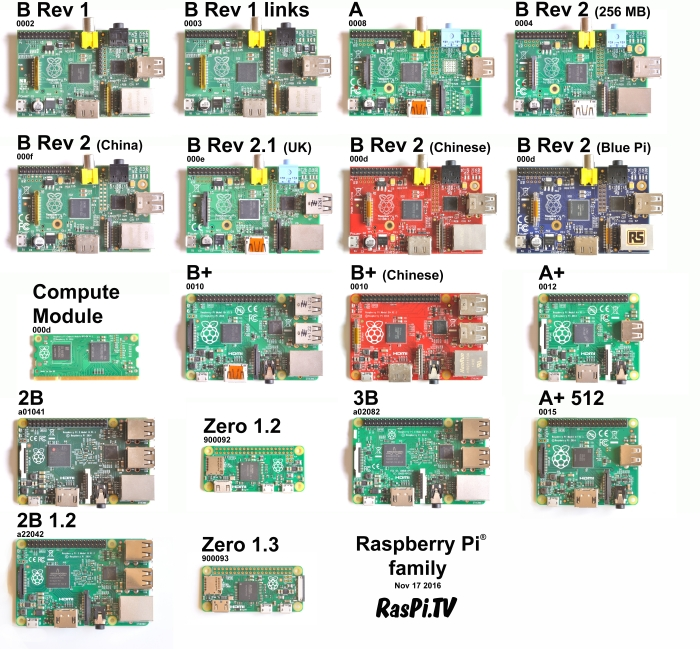
\includegraphics{images/pi-family}
	\caption{Les différents modèles de Pi}
	\label{img_family}
\end{figure}
\end{center}

\end{frame}

\section{Les caractéristiques du Pi 3}

\begin{frame}
\frametitle{Le Raspberry Pi 3}

Broadcomm est censé avoir libéré toutes les spécifications des circuits depuis 2014.

Le CPU est de la famille ARMv8 et est donc un processeur RISC. Vous retrouverez des ARM un peu partout maintenant puisque c'est le processeur le plus fréquent pour les smartphones, tablettes et autres joujous. Celui du Raspberry Pi 3 a quatre coeurs Cortex A53.

Il est 64 bits et compatible 32 bits. Toutefois il est bridé pour l'instant car le support 64 bits n'est apparu que dans une des dernières versions du kernel Linux. Pour l'instant avec la Raspbian, il est encore bridé en 32 bit.

\end{frame}

\begin{frame}
\frametitle{Le Raspberry Pi 3}

Le GPU est quant à lui un VideoCore IV double coeur. Il est compatible OpenGL et supporte l'accélération matérielle~: certains calculs 2D peuvent être déportés sur le GPU par le CPU.

Il possède un accélération matérielle pour ce qui est codé en H.264. Il supporte aussi le MPEG-2 et le VC-1 mais pour les utiliser il faut acheter une licence. Licence qui est associée au numéro de processeur du Pi.
\end{frame}

\begin{frame}
\frametitle{Le Raspberry Pi 3}
Un composant spécifique gère à la fois le LAN et l'USB ce qui peut éventuellement générer un engorgement.

Les composant WiFi et Bluetooth sont pratiques mais ils n'ont une portée que d'une dizaine de mètres contrairement aux clefs USB qui ont une portée plus proche des 30m pour le WiFi.
\end{frame}

\begin{frame}
\frametitle{Le Raspberry Pi 3}

Un détail qui a son importance, le Raspberry Pi n'a pas d'horloge interne. Elle se mets à l'heure grâce à un serveur sur Internet. C'est utile de le savoir pour certaines applications.

Pour une somme modique des horloges internes sont disponibles à brancher sur le port GPIO.

\end{frame}
